\documentclass[a4paper,10pt]{article}
\usepackage[utf8]{inputenc}
\usepackage{amsmath}
\usepackage{graphicx}
\usepackage{float}
\usepackage{rotating}

\usepackage{todonotes}

\title{}
\author{}

\begin{document}
	\section{Project Description - Rotating LED Display}
	The purpose of this project is to create an LED strip which, when rotating will create a display-like effect by utilizing persistence of vision.
	The components to be created for this project are:
	\begin{itemize}
		\item \textbf{LED board:} A PCB must be designed which houses the LEDs as well as the driver circuitry.
		\item \textbf{Communication component:} This component will maintain the communication with the LED driver.
		\item \textbf{Graphics component:} This component should include the logic required to display a stable image.
		\item \textbf{Motor component:} This component will, by using the encoder output of the dc motor, maintain a steady speed of the motor.
		\item \textbf{Power Supply:} The power supply from the brick sorter will be reused in this project.
		\item \textbf{$\mu$TosNet:} $\mu$TosNet will be used for debugging purposes.
		Potentially, it will also be used to send a string to display as an image.
	\end{itemize}
	Initially, the goal of the project will be to display the image shown in figure \ref{fig:circle}. 
	By displaying this image stably and with the 90 degree angles intact a descent foundation for further graphics display is laid.
	
	\begin{figure}[h!]
		\centering
		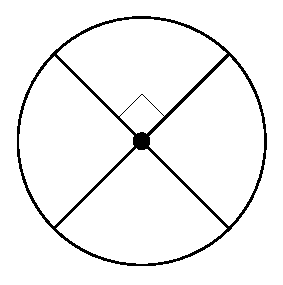
\includegraphics[width=.25\linewidth]{images/circle}
		\caption{Initial test image of the rotating display}
		\label{fig:circle}
	\end{figure}
	
	The initial model of the system can be seen in figure \ref{fig:initmodel}. As can be seen, the led board which contains the driver circuit receives information about the state of the LEDs from the communication component in the FPGA. The graphics to be displayed is generated in the graphics component, potentially based on input from $\mu$TosNet. Additionally, the graphics component is given information about the speed of the motor in order to correctly display the image.
	
	\begin{figure}[h!]
		\centering
		\includegraphics[width=.7\linewidth]{images/init_model}
		\caption{Simple block diagram showing the different components of the system, and their interactions.}
		\label{fig:initmodel}
	\end{figure}
		
	\newpage
	
	\begin{sidewaystable}[h!]
		\begin{tabular}{l|c|c|c|c}
			Company & Order Number & Quantity & Name & Price/1\\
			\hline
			RS-Components & 708-0725 & 30 & Osram Opto RGB LED & 2.812Dkk\\
			\hline
			RS-Components & 789-3830 & 4 & 16ch con.current LED Driver 0.1A SOIC-24 & 12.072Dkk\\
			\hline
			RS-Components & 238-9709 & 1 & DC motor, Speed: 7800 o/min., 1,6 W, 15 - 3 V=, 0,85 A & 47.74Dkk\\
			\hline
			Sparkfun & & 1 & Slip Ring - 12 Wire (2A) & 19.95\$
			& & & &
		\end{tabular}
	\end{sidewaystable}
\end{document}